\renewcommand{\baselinestretch}{2} \small\normalsize
\section{Propagation Modeling}
This chapter describes how propagation is modeled for this effort.

\subsection{Analytical Approach}
From \cite{frazier_green}, we can derive asymptotic solutions for the wave reflected from the surface using both paraxial and cylindrical waves as shown in Figure \ref{prop_fig:0}. Here we see that the results can be broken up into the product of 3 components: a geometric spreading term, the plane wave solution, and a sum of Bessel functions that describes the random portion. 

\begin{figure}[H]
  \begin{center}
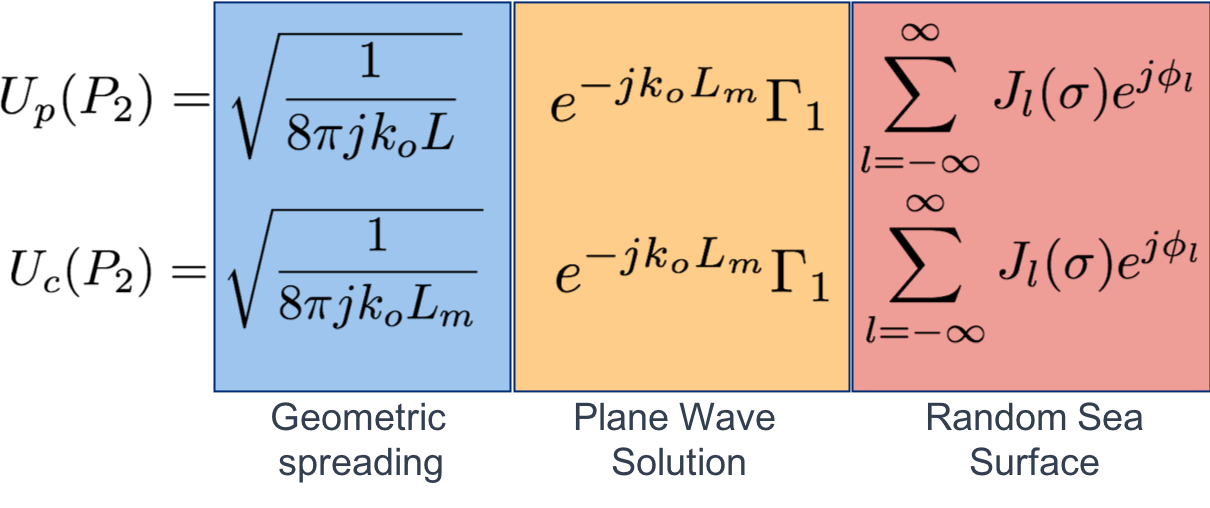
\includegraphics[width=4in]{../media/multistatic/analytical_solutions.png}
  \end{center}
  \renewcommand{\baselinestretch}{1} \small\normalsize
  \begin{quote}
    \caption[Asymptotic Solutions for the Reflected Rays]{Asymptotic Solutions for the Reflected Rays\label{prop_fig:0}}
  \end{quote}
\end{figure}
\renewcommand{\baselinestretch}{2} \small\normalsize

The only difference between the paraxial and cylindrical wave solutions is in the geometric spreading term. For the paraxial case, the spreading is dependent on the projected path length in the direction of propagation ($L$) while for the cylindrical case, the spreading is dependent on the total path length ($L_m$). 

For propagation, we are more interested in the propagation factors, which are given for the paraxial wave case as \cite{frazier_green}:

\begin{equation}
F_p =e^{-jk_oL_1}+\Gamma_1 e^{-jk_oL_m} \sum_{l=-\infty}^{\infty}J_l(\sigma)e^{j\phi_l}
\label{prop_eq:1}
\end{equation}
\renewcommand{\baselinestretch}{2} \small\normalsize

\noindent The propagation factors for the cylindrical wave case are given as \cite{frazier_green}:

\begin{equation}
F_p =e^{-jk_oL_1}+\Gamma_1\sqrt{\frac{L_1}{L_m}} e^{-jk_oL_m} \sum_{l=-\infty}^{\infty}J_l(\sigma)e^{j\phi_l}
\label{prop_eq:2}
\end{equation}
\renewcommand{\baselinestretch}{2} \small\normalsize

\noindent The intermediate variables for Equations \ref{prop_eq:1} and \ref{prop_eq:2} are given in Equation \ref{prop_eq:3}.

\begin{equation}
\begin{gathered}
L_m = L + \frac{(h_1+h_2)^2}{2L} \\
L_0''=\frac{(h_1+h_2)^4}{h_1h_2L^3} \\
\sigma = \frac{2k_os(h_1+h_2)}{L} \\
\phi_l = l\theta - \frac{l^2k_{\omega}^2}{2k_oL_0''}
\label{prop_eq:3}
\end{gathered}
\end{equation}
\renewcommand{\baselinestretch}{2} \small\normalsize

\subsection{Numerical Approach}
The analytical approach simplifies the problem by treating diffraction from the sea surface in plane so that integration is done downrange. This requires additional approximations and constraints, so a more accurate method is to integrate in altitude and march the solution in range. This approach is well suited to the Fourier Split-Step technique given by \cite{frazier_green} as

\begin{equation}
A(x,z) = \exp\left[-j\frac{k_pm}{2}\Delta x\right]\mathcal{F}^{-1}\left\{\exp\left[j\frac{k_z^2}{2k_p}\Delta x \right]\hat{A}(x_o,k_z) \right\}
\label{prop_eq:4}
\end{equation}
\renewcommand{\baselinestretch}{2} \small\normalsize

APL's Tropospheric Electromagnetic Parabolic Equation Routine (TEMPER) \cite{temper_guide} provides a validated tool for RF propagation that implements the Fourier Split-Step algorithm and is used for numerical propagation in this work.

